%
% File: chap02.tex
%
\let\textcircled=\pgftextcircled
\chapter{Theory and conceptual framework}
\label{Chapter2}

\section{Preliminaries}
Description of concepts

%%%%%%%%%%%%%%%%%%%%%%%%%

\begin{definition}
orthogonal complement
\end{definition}

\begin{theorem}
	For every $n\times n$ symmetric real matrix, the eigenvalues are real and the eigenvectors can be chosen real and orthonormal.
\end{theorem}

\begin{theorem}[Courant-Fisher Formula]
Let $A$ be an $n\times n$ real symmetric matrix with eigenvalues $\lambda_1 \leq \lambda_2 \leq \cdots \leq \lambda_n$ and corresponding eigenvectors $v_1, v_2,..., v_n$. Then 
\begin{align*}
	\lambda_1 &= \min_{\left \Vert x\right\Vert = 1} x^TAx = \min_{ x \neq 0} \frac{x^TAx}{x^Tx}, \\
	\lambda_2 &= \min_{\substack{\left \Vert x\right\Vert = 1 \\ x\perp v_1}} x^TAx = \min_{ x \neq 0} \frac{x^TAx}{x^Tx}, \\
	\lambda_n &= \lambda_{\text{max}} = \max_{\substack{\left \Vert x\right\Vert = 1 \\ x\perp v_1}} x^TAx = \max_{\substack{ x \neq 0 \\ x\perp v_1}} \frac{x^TAx}{x^Tx}.
\end{align*}
In general, for $1\leq k \leq n$, let $S_k$ denote the span of $v_1, v_2,..., v_k$ (with $S_0=\{0\}$). Then 
\begin{displaymath}
	\lambda_k = \min_{\substack{\left \Vert x\right\Vert = 1 \\ x\in S_{k-1}^\perp}} x^TAx = \min_{\substack{x \neq 0 \\ x\in S_{k-1}^\perp}} \frac{x^TAx}{x^Tx}.
\end{displaymath}
\end{theorem}
%\begin{proof}
%	Let $A=Q\Lambda Q^T$ be the eigenvalue decomposition of $A$, where $Q$ is an orthogonal matrix whose columns are %eigenvectors of $A$, and $\Lambda$ is a diagonal matrix whose entries are the eigenvalues of $A$.
%\end{proof}

\section{Graphs and Laplacian Matrices}
For the rest of the chapter, let $G=(V,E)$ be a graph, where $V=\left\{v_1, v_2, ... , v_n\right\}$ is the non-empty set of nodes (or vertices) and $E$ is the set of edges, composed by pairs of the form $(v_i, v_j)$, where $v_i, v_j \in V$.

It is assumed that all graphs are undirected, meaning that if $(v_i, v_j)\in E$, then $(v_j, v_i)\in E$, for every $v_i,v_j \in V$. For that reason, the edge $(v_i, v_j)$ will be represented as the unordered set $\left\{ v_i, v_j\right\}$.

    A convenient way to represent a graph is through an \textit{adjacency matrix} $A\in\mathbb{R}^{\left|V\right|\times\left|V\right|}$. Giving a specific order to the graph nodes, one can represent the edges as binary entries in this matrix:
    \begin{displaymath}
        A[v_i, v_j] = 
        \begin{cases}
            1 & \text{if } \left\{ v_i, v_j\right\}\in E \\
            0 & \text{otherwise}
        \end{cases}
    \end{displaymath}
    
    Let $\EuScript{N}(v_i)$ denote the neighborhood of node $v_i$, i.e., the set of the adjacent nodes to it. The quantity that represents the number of nodes in $\EuScript{N}(v_i)$ is called the \textit{degree of the vertex} $v_i$. This is one of the most obvious and informative feature for the structure of the graph and is denoted by
	\begin{displaymath}
		d_i = \sum_{j=1}^n A[v_j, v_i].
	\end{displaymath}
	
	Finally, we can summarize that graph's information in the \textit{degree matrix} $D$ which is defined as the diagonal matrix with the degrees $d_1, d_2, ..., d_n$ on the diagonal.
	
\subsection{The Unnormalized Laplacian}
	The unnormalized graph \textit{Laplacian matrix} $L$ is defined as 
	\begin{displaymath}
		L = D - A
	\end{displaymath}
	
	\begin{proposition}[Some properties of $L$]
	    The matrix $L$, as defined above, satisfies the following properties:
	    \begin{enumerate}
	    	\item For every vector $x=(x_1,x_2, ..., x_n)\in \R$ we have 
	    	\begin{displaymath}
	    		%x^TLx = \frac{1}{2}\sum_{i=1}^n\sum_{j=1}^n w_{ij}\left(x_i-x_j\right)^2
	    		x^TLx = \frac{1}{2}\sum_{i=1}^n\sum_{j=1}^n \left(x_i-x_j\right)^2
	    	\end{displaymath}
	    	\item $L$ is symmetric and positive semi-definite
	    	\item $L$ has $n$ non-negative, real-valued, eigenvalues $\lambda_1 \leq \lambda_2 \leq \cdots \leq \lambda_n$
		    \item The smallest eigenvalue of $L$ is $0$, the corresponding eigenvector is the constant one vector $\mathbb 1$.
	    \end{enumerate}
    \end{proposition}
 
\subsection{Normalized Laplacians}
	The \textit{symmetric normalized Laplacian} matrix $L_{sym}$ is defined as
	\begin{displaymath}
		L_{sym} = D^{-\frac{1}{2}}LD^{-\frac{1}{2}}
	\end{displaymath}
	while the \textit{random walk Laplacian} is defined as 
	\begin{displaymath}
		L_{rw} = D^{-1}L
	\end{displaymath}

%\begin{definition}
%	For a collection of vertices $A\subset V$, we define the \textbf{edge boundary} of $A$ as
%	\begin{displaymath}
%		\partial(A)=\left\lbrace (u,v)\in E \mid  u\in A, v\in \overline{A} \right\rbrace
%	\end{displaymath}
%\end{definition}

\subsection{The graph partitioning problem}
In order to introduce the graph partitioning problem in its different settings, the mathematical definition of the concepts involved are presented below.
\begin{definition}
	Given a graph $G = (V, E)$ and an integer $K$, a \textit{partition} of $G$ is a collection of $K$ subsets $P_1, P_2, ..., P_K\subset V$ such that:
	\begin{enumerate}
		\item $P_i \cap P_j = \emptyset$ for $i\neq j$, where $i,j\in \{1,2,...,K\}$
		\item $\cup_{k=1}^K P_k = V$
	\end{enumerate}	 
\end{definition}
    A partition of a graph can be seen as simply removing edges from the original graph in such way the obtained partitions are subgraphs. There are many ways a graph can be partitioned into subgraphs and the way it gets done depends completely on the application of interest. However, independently of the problem to solve, the objective relies on minimizing the connections between the partitions in the original graph. The following concepts provides a useful notation to turn the problem into an optimization one.
    
	For a collection $S\subset V$ of vertices, we define the \textit{edge boundary} $\partial(S)$ to consist of all edges in $E$ with exactly one endpoint in $S$, that is,
	\begin{displaymath}
		\partial(S) := \left\{ \left\{u, v\right\}  \in E \mid u \notin S \text{ and } v\in S \right\}
	\end{displaymath}
	
	Now the problem turns into finding a partition $P_1, P_2, ..., P_K$ such that minimizes the \textit{cut value} of the partition, usually called just \textit{cut}, which is defined as
	\begin{equation}
	    \label{mincut}
	    \textsc{Cut}(P_1, P_2, ..., P_K) := \frac{1}{2} \sum_{k=1}^K \left|\partial(P_k)\right|
	\end{equation}
	
	The notion of cut allows to measure the quality of any partition, nevertheless solving the min cut problem ...

	For a collection of vertices $S\subset V$, consider the following quantities related to the edges of 
	
	\begin{displaymath}
		\textsc{Vol}(S) :=  \sum_{v_i \in S} d_i 
	\end{displaymath}

 
we want to agroupe by similarity so its natural to 
Cut value of that partition

solve the mincut problem

The next consider two different ways of measuring the size of the partitions
\begin{align*}
	\textsc{RatioCut}(P_1, P_2, ..., P_K) &:= \frac{1}{2} \sum_{k=1}^K \frac{\left|\partial\left(P_k\right)\right|}{\left| P_k \right|} \\
	&= \sum_{k=1}^K \frac{\textsc{Cut}(P_k, \overline{P_k})}{\left| P_k \right|}
\end{align*}

\begin{align*}
	\textsc{NormCut}(P_1, P_2, ..., P_K) & := \frac{1}{2} \sum_{k=1}^K \frac{\left|\partial\left(P_k\right)\right|}{\textsc{Vol}(P_k)}\\
	&= \sum_{k=1}^K \frac{\textsc{Cut}(P_k, \overline{P_k})}{\textsc{Vol}(P_k)}
\end{align*}

%%%%%%%%%%%%%%%%%%%%%%%%%%%%%%%%%%%%%%%%%%%%%%%%%%%%%%%%%%%%%%%%%%%%%%%%%%%%%5
\begin{comment}
\textbf{The spectral method}
\begin{enumerate}
	\item Let $v$ denote the second smallest eigenvector of $\mathcal{L}$. Sort the vertices $i$ of $G$ in increasing order of $v_i$. Let the resulting ordering be $v_1 \leq v_2 \leq \cdots v_n$
	\item For each $i$, consider the cut induced by $\{1,2,..., i\}$ and its complement. Calculate its conductance.
	\item Among these $n-1$ cuts, choose the one with minimum conductance.
\end{enumerate}

\textbf{Cheeger's inequality}

For a graph $G=(V,E)$ the \textit{conductance} or \textit{Cheeger ratio} of a set $S\subset V$ is the ratio of the fraction of edges in the cut $(S,\overline{S})$ o the volume of $S$,
\begin{displaymath}
	\phi(S) = \frac{E(S,\overline{S})}{\textsc{Vol}(S)}
\end{displaymath}

The \textit{conductance} or \textit{Cheeger constant} of a graph $G$ is denoted by 
\begin{displaymath}
	\phi(G) = \min_S \phi(S)
\end{displaymath}

\begin{theorem}
	In a graph $G$, the Cheeger constant $\phi(G)$ and the spectral gap $\lambda_G$ are related as follows:
	\begin{displaymath}
		2\phi(G)\geq \lambda_G \geq \frac{\alpha_G^2}{2} \geq \frac{\phi(G)^2}{2} 
	\end{displaymath}
	where $\alpha_G^2$ is the minimum Cheeger ratio of subsets $S_i$ consisting of vertices with the largest $i$ values in the eigenvector associated with $lambda_G$ , over all $i\in[n]$
\end{theorem}

\textbf{Generalization to many partitions}
\begin{enumerate}
	\item Perform eigenvalue decomposition to find the eigenvectors of $L_{sym}$.
	\item Select the $k$ largest eigenvectors $e_1, e_2, ..., e_k$ of $L_{sym}$ associated to the largest eigenvalues $\lambda_1, \lambda_2, ..., \lambda_k$
	\item Form the matrix $Y$ from the matrix $X=[e_1, e_2,..., e_k]$ given by 
	\begin{displaymath}
		Y_{ij} = \frac{X_{ij}}{\left(\sum_j X_{ij}^2\right)^\frac{1}{2}}
	\end{displaymath}
	\item Treating each row of $Y$ as a point in $\mathbb R^k$, cluster them into $k$ clusters using $K-means$
	\item Finally, assign the original vertex to cluster $j$ if and only if row $i$ of the matrix was assigned to cluster $j$
\end{enumerate}
\end{comment}
%%%%%%%%%%%%%%%%%%%%%%%%%%%%%%%%%%%%%%%%%%%%%%%%%%%%%%%%%%%%%%%%%%%%%%%%%%%%%%%%%%%%

\subsection{Spectral partitioning and Normalized Cut}
Here will be presented the derivation of the normalized cut as relaxation of the problem to solve the spectral partitioning problem

\section{Literature review}

B-GRAP: BALANCED GRAPH PARTITIONING ALGORITHM
FOR LARGE GRAPHS:
https://www.rintonpress.com/xjdi2/xjdi2-2/116-135.pdf

Trading Quality for Efficiency of Graph Partitioning: An Inductive Method across Graphs 
https://openreview.net/forum?id=e6MWIbNeW1

Application Driven Graph Partitioning
https://dl.acm.org/doi/abs/10.1145/3318464.3389745

Graph Partitioning and Sparse Matrix Ordering using Reinforcement Learning~\cite{nesteddissection}


\subsection{Generalizable Approximate Graph Partitioning (GAP) Framework}
From all the Deep Learning approaches that solve the Graph Partitioning problem, one of the most notorious not only for its simplicity but for its exceptional results, is the \textit{Generalizable Approximate Graph Partitioning} framework better known as GAP~\cite{gap1}.

GAP is a Graph Neural Network approach that proposes a continuous relaxation of the problem using a differentiable loss function that is based on the normalized cut. According to Nazi et al.~\cite{gap}, it is an unsupervised learning algorithm that is capable of generalization, meaning that it can be trained in small graphs, which allows it to generalize into unseen much larger ones. This section describes the model described in the original paper which consists of two modules: the Graph Embedding Module and the Graph Partitioning Module. See Figure~\ref{fig:gap}.

\begin{figure}[h!]
    \begin{center}
        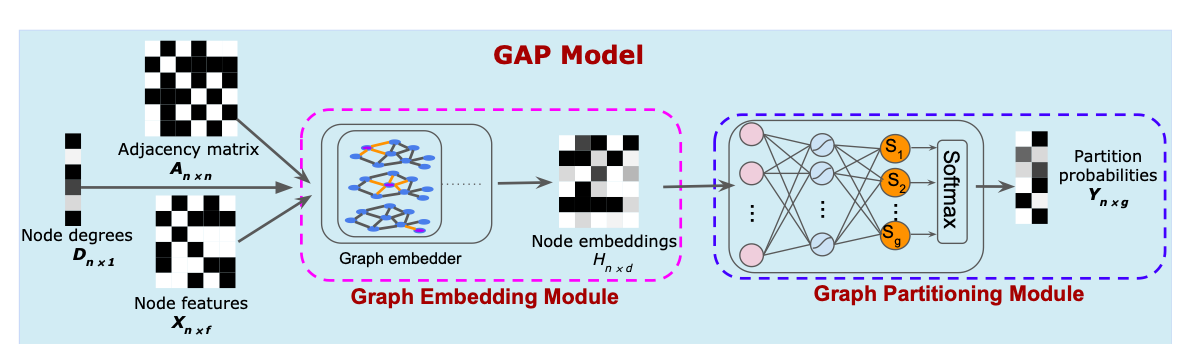
\includegraphics[scale=0.38]{GAP.png}
    \end{center}
    \caption{Architecture of the Generalizable Approximate Partitioning framework~\cite{gap}.}
    \label{fig:gap}
\end{figure}

In the following subsections, it is assumed that the framework takes a graph $G = (V, E)$ as input, where $V = \left\{ v_1, v_2, ..., v_n\right\}$, and outputs the probabilities tensor $Y\in \mathbb R^{n\times K}$, where $Y_{ik}$ represents the probability that node $v_i$ belongs to partition $P_k$. %being $P_1, P_2, ..., P_k$ 
Before going into the model description, the deduction of the loss function is as follows.

\subsubsection{Expected Normalized Cut Loss Function}
Recall the normalized cut given by
\begin{equation}
    \label{eq:normalized_cut}
        \textsc{NormCut}(P_1, P_2, ..., P_K) = \sum_{k=1}^K \frac{\textsc{Cut}(P_k, \overline{P_k})}{\textsc{Vol}(P_k)}
\end{equation}
    
In order to calculate the normalized cut expected value, one needs to compute the expected value of $\textsc{Cut}(P_k, \overline{P_k})$ and $\textsc{Vol}(P_k)$ from Equation~\ref{eq:normalized_cut}. For the deduction of those quantities, an approach similar to the one presented in~\citep{gap2} will be followed .

Since $Y_{ik}$ represents the probability that node $v_i\in P_k$, $1 - Y_{ik}$ is the probability that $v_i\notin P_k$, hence 
\begin{equation}
    \label{eq:first_expected_cut}
    \mathbb{E}[\textsc{Cut}(P_k, \overline{P_k})] = \sum_{i=1}^{|V|} \sum_{v_j\in\EuScript{N}(v_i)} Y_{ik}(1-Y_{jk})
\end{equation}
as can it can be deducted from Figure~\ref{fig:expectation}.

Due to the fact that for a given node the adjacent nodes can be retrieved from the adjacency matrix $A$, Equation~\ref{eq:first_expected_cut} can be rewritten as follows:
\begin{equation}
    \label{eq:expected_cut}
    \mathbb{E}[\textsc{Cut}(P_k, \overline{P_k})] = \sum_{i=1}^{|V|}\sum_{j=1}^{|V|}Y_{ik}(1-Y_{kj}^T)A_{ij} 
\end{equation}

\begin{figure}[h!]
    \begin{center}
        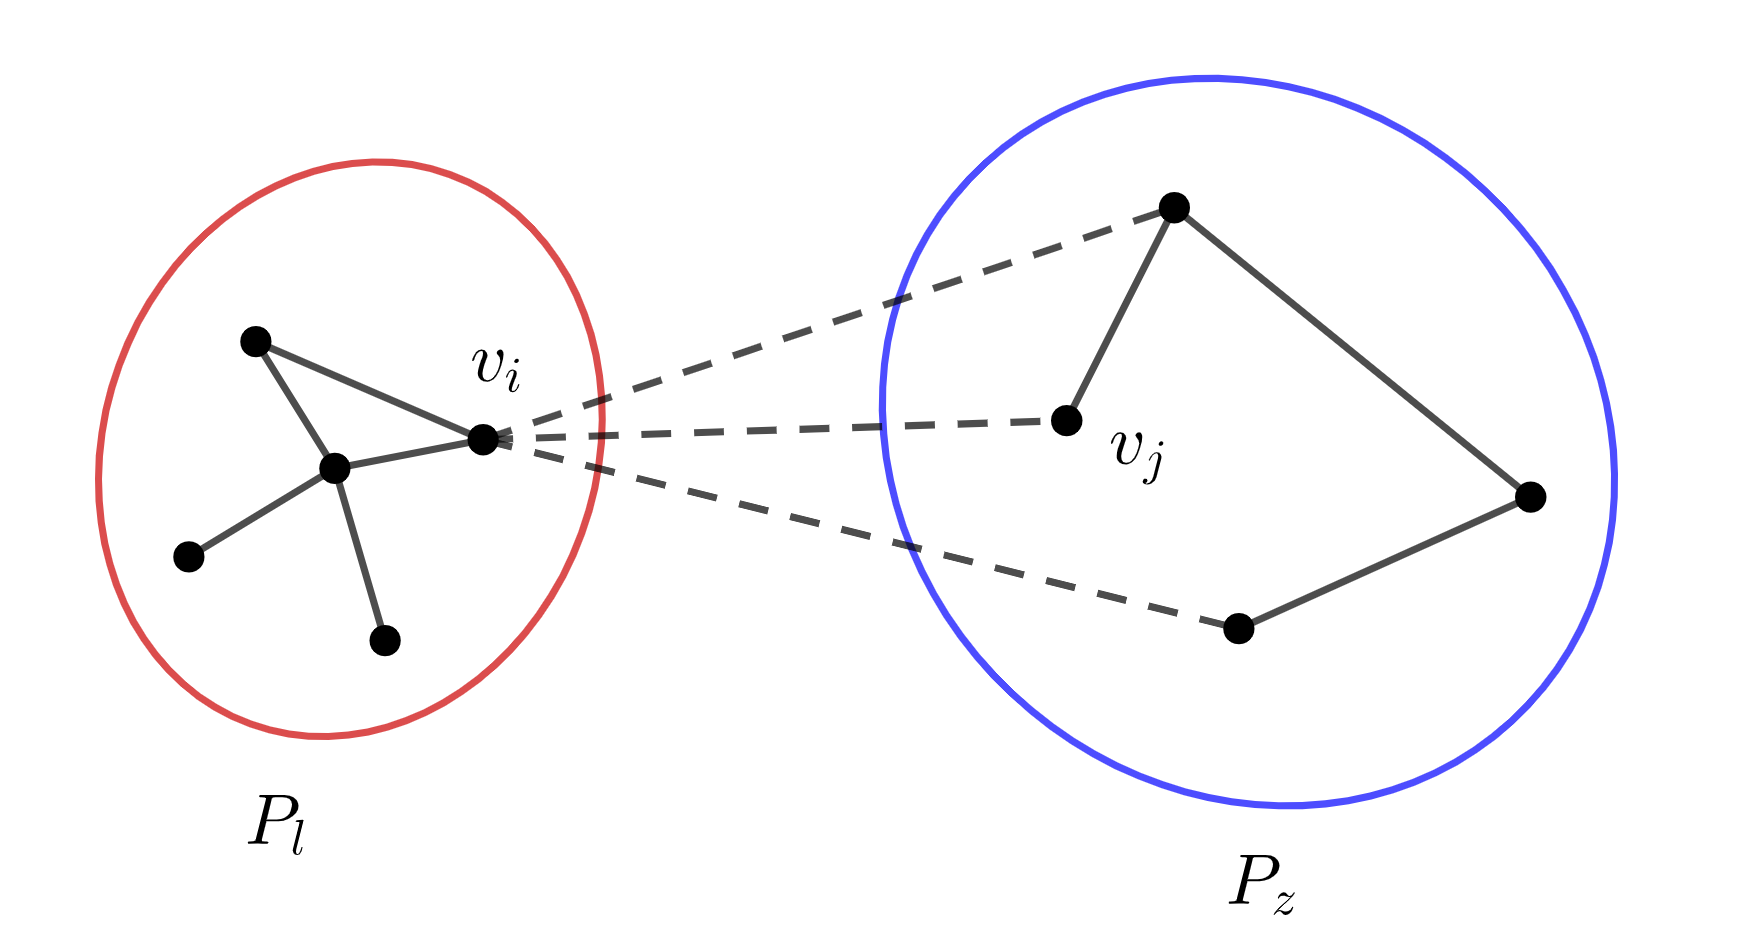
\includegraphics[scale=0.7]{expectation.png}
    \end{center}
    \caption{The expected value of the number of edges in the boundary of a determined partition $P_l$ is given by the sum of the probabilities that each node $v_i\in V$ belongs to $P_l$, multiplied by the probability that each of its neighbors does not belong to $P_l$.}
    \label{fig:expectation}
\end{figure}

Keeping in mind that $\textsc{Vol}(P_k)$ is the sum of the degrees of the nodes in $P_k$, $\Delta$ is defined to be the column tensor where $\Delta_i$ is the degree of the node $v_i\in V$. Then, given $Y$, one can calculate the expected value of $\textsc{Vol}(P_k)$ as follows:
\begin{equation}
    \label{eq:expected_vol}
    \begin{split}
        \Gamma &= Y^T\Delta \\
        \mathbb{E}[\textsc{Vol}&(P_k)] = \Gamma_k
    \end{split}
\end{equation}

From the results obtained in Equation~\ref{eq:expected_cut} and Equation~\ref{eq:expected_vol}, a way to calculate the expected value of $\textsc{NormCut}(P_1, P_2, ..., P_K)$ is given by:
\begin{equation}
    \label{eq:expected_norm_cut}
    \mathbb{E}[\textsc{NormCut}(P_1, P_2, ..., P_K)] = \sum_{k=1}^K\sum_{i=1}^{|V|}\sum_{j=1}^{|V|}\frac{Y_{ik}(1-Y_{kj}^T)A_{ij}}{\Gamma_k}
\end{equation}

Nazi et al.~\cite{gap} also showed that given the probability tensor $Y$, one can evaluate how balanced those partitions are.
Note that the sum of the columns in $Y$ is the expected number of nodes in each partition, i.e., $\mathbb{E}[|P_k|]=\sum_{i=1}^{|V|}Y_{ik}$. On the other hand, in order to have balanced partitions, the number of nodes in each one should be $\frac{|V|}{K}$. As a consequence, the quantity $\left|\sum_{i=1}^{|V|}Y_{ik} - \frac{|V|}{K}\right|$ measures how balanced the partition $P_k$ is.

Using the last result, and replacing the absolute value by the squared function, one can derive the loss function from Equation~\ref{eq:expected_norm_cut}. This is the one originally used in GAP that intends to minimize the expected value of the normalized cut and at the same time balances the cardinalities of the partitions:

\begin{equation}
    \label{eq:loss_function}
    \mathcal{L} = \sum_{k=1}^K\sum_{i=1}^{|V|}\sum_{j=1}^{|V|}\frac{Y_{ik}(1-Y_{kj}^T)A_{ij}}{\Gamma_k} + \sum_{k=1}^K\left(\sum_{i=1}^{|V|}Y_{ik} - \frac{|V|}{K}\right)^2
\end{equation}

\subsubsection{The Embedding Module} In the graph embedding module, the algorithm learns node embeddings by encoding local structure information and the node features. The embeddings are calculated using Graph Neural Networks (GNN) which have become very popular during the recent years. To ensure generalization, the GAP authors opted for an inductive GNN approach by leveraging GraphSAGE with a Graph Convolutional Network (GCN) based approach.

In the paper where GAP was presented, the authors used a $3$-layer GCN using Xavier initialization that can be found in~\cite{xavier}
\begin{displaymath}
    Z = \tanh(\hat{A}\tanh(\hat{A}\tanh(\hat{A}X\boldsymbol W^{(0)})\boldsymbol W^{(1)})\boldsymbol W^{(2)})
\end{displaymath}
where $\hat{A} = (D+I)^{-\frac{1}{2}}(A+I)(D+I)^{-\frac{1}{2}}$ is a normalized variant of the adjacency matrix with self loops, $X$ is the feature matrix, and $\boldsymbol W^{(l)}$ is a learnable parameter matrix.

\subsubsection{The Partitioning Module}
The second module of GAP is composed of a fully connected layer that takes as input a node embedding vector $\boldsymbol z_u$ generated in the embedding module. This fully connected layer is then followed by a softmax layer 
trained to minimize the expected normalized loss function given by Equation~\ref{eq:loss_function}.

\begin{figure}[h!]
    \label{fig:partitioning_module}
    \begin{center}
        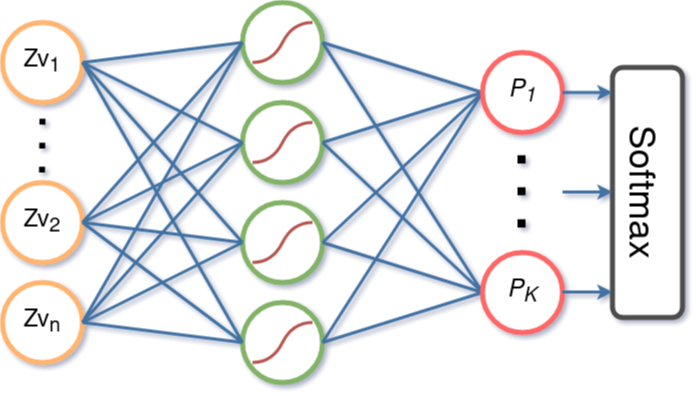
\includegraphics[scale=0.5]{partitioning_module}
    \end{center}
    \caption{The partitioning module. A dense neural network that processes a node embedding and outputs the probability of the corresponding node to belong to each partition.}
\end{figure}
\newpage
This module is the responsible for partitioning the graph by returning $Y\in \mathbb R^{|V|\times K}$, the probabilities matrix that each node belongs to each of the partitions $P_1, P_2, ..., P_K$. At the same time, it ensures that for a given node, the sum of the probabilities of belonging each of the partitions is $1$
\begin{displaymath}
    \sum_{k=0}^K Y_{ik} = 1
\end{displaymath}


